% !TEX TS-program = pdflatex
% !TEX encoding = UTF-8 Unicode

% This is a simple template for a LaTeX document using the "article" class.
% See "book", "report", "letter" for other types of document.

\documentclass[11pt]{report} % use larger type; default would be 10pt

\usepackage[utf8]{inputenc} % set input encoding (not needed with XeLaTeX)
\usepackage{amsmath}


%%% Examples of Article customizations
% These packages are optional, depending whether you want the features they provide.
% See the LaTeX Companion or other references for full information.

%%% PAGE DIMENSIONS
\usepackage[margin=0.5in]{geometry} % to change the page dimensions
\geometry{a4paper} % or letterpaper (US) or a5paper or....
% \geometry{margin=2in} % for example, change the margins to 2 inches all round
% \geometry{landscape} % set up the page for landscape
%   read geometry.pdf for detailed page layout information

\usepackage{graphicx} % support the \includegraphics command and options

% \usepackage[parfill]{parskip} % Activate to begin paragraphs with an empty line rather than an indent

%%% PACKAGES
\usepackage{booktabs} % for much better looking tables
\usepackage{array} % for better arrays (eg matrices) in maths
\usepackage{paralist} % very flexible & customisable lists (eg. enumerate/itemize, etc.)
%\usepackage{verbatim} % adds environment for commenting out blocks of text & for better verbatim
\usepackage{subfig} % make it possible to include more than one captioned figure/table in a single float
% These packages are all incorporated in the memoir class to one degree or another...

%%% HEADERS & FOOTERS
\usepackage{fancyhdr} % This should be set AFTER setting up the page geometry
\pagestyle{fancy} % options: empty , plain , fancy
\renewcommand{\headrulewidth}{0pt} % customise the layout...
\lhead{}\chead{}\rhead{}
\lfoot{}\cfoot{\thepage}\rfoot{}

%%% SECTION TITLE APPEARANCE
\renewcommand\thesection{\arabic{section}}
\renewcommand\thesubsection{\thesection.\arabic{subsection}}
\usepackage{sectsty}
\allsectionsfont{\sffamily\mdseries\upshape} % (See the fntguide.pdf for font help)
% (This matches ConTeXt defaults)

%%% ToC (table of contents) APPEARANCE
\usepackage[nottoc,notlof,notlot]{tocbibind} % Put the bibliography in the ToC
\usepackage[titles,subfigure]{tocloft} % Alter the style of the Table of Contents
\renewcommand{\cftsecfont}{\rmfamily\mdseries\upshape}
\renewcommand{\cftsecpagefont}{\rmfamily\mdseries\upshape} % No bold!

\usepackage{natbib}
\setlength{\bibsep}{0pt}

\usepackage[english]{babel}

%------------------------
%Uncomment below to reduce space after Bibliography
%\usepackage{titlesec}
%\titleformat{\chapter}[display]
%    {\normalfont\huge\bfseries}{\chaptertitlename\ \thechapter}{20pt}{\Huge}
%\titlespacing*{\chapter}{0pt}{50pt}{10pt}
%------------------------

\usepackage{caption}
\usepackage{import}

%------------------------
%For positioning images and to have a box around them
%------------------------
\usepackage{float}
%\floatstyle{boxed} 
\restylefloat{figure}
\usepackage{subfloat}
\setlength{\fboxsep}{1mm} %padding thickness for boxes around images
\setlength{\fboxrule}{1pt} %border thickness for boxes around images
\usepackage{sidecap}	%To display text next to images
\usepackage{wrapfig}	%To wrap text around images
%------------------------

%------------------------
% Multi-line comment
%------------------------
\newcommand{\comment}[2]{#2}

%%% END Article customizations

%%% The "real" document content comes below...

%###################################################################################

\title{Analysis of Garbage Collector Algorithms in Non-Volatile Memory Devices}
\author{{Ananth Mahadevan$^\dagger$$\oplus$}\\
email: {\texttt{\{mahadeva\}}}@cse.ohio-state.edu\\
$^\dagger$ The Ohio State University, Columbus, OH \\
$\oplus$ The Samraksh Company, Dublin, OH \\
}

%\author{The Samraksh Company}
%\numberofauthors{4}
%\author{Ananth Mahadevan, Dr. Mukundan Sridharan, Dr. Kenneth W Parker, Dr. Rajiv Ramnath}\\

%\author{{Ananth Mahadevan$^\dagger$$\oplus$, Mukundan Sridharan$\oplus$,  Kenneth W Parker$\oplus$, Rajiv Ramnath$^\dagger$}\\
%email: {\texttt{\{mahadeva\}}, {\{Ramnath\}}}@cse.ohio-state.edu\\
%email: {\texttt{\{Mukundan.Sridharan\}}, {\{Kenneth.Parker\}}}@Samraksh.com\\
%$\oplus$ The Samraksh Company \\
%$^\dagger$ The Ohio State University \\
%}

%\date{} % Activate to display a given date or no date (if empty),
         % otherwise the current date is printed 

\DeclareMathSizes{11}{19}{13}{9}

\begin{document}
\maketitle

\makeatletter
\renewcommand\section{\@startsection {section}{1}{\z@}%
    {-3.5ex \@plus -1ex \@minus -.2ex}%
    {2.3ex \@plus.2ex}%
    {\normalfont\large\bfseries}}
\makeatother

%--------------------------------------------------------------------------------------------------------
%\begin{center}
\section*{FOREWORD}
	This work is dedicated to my father Sri.N.Mahadevan.

As I was writing this report, I started thinking about so many things I am grateful for in my life. Wonderful parents and brother. Friends and family who stuck with us during times of trouble and shared our moments of happiness. Thanks to my grandparents, uncles, aunts, cousins and of course friends. 

A special mention about Dr.M.B.Anand who sowed the thought  of doing my Masters in my head. 

Thirukkural: 396
The deeper you dig, greater the spring;
The more you learn, greater the knowledge

\end{center}

\tableofcontents

\section{Abstract}
	The performance results for five different Garbage Collection (GC) algorithms for Non-Volatile Memory Devices for three access patterns are presented in this report. The access patterns include a long-tailed distribution as well as Uniform distribution. The results indicate that Round-Robin style GC algorithms perform much better in all cases than Generational algorithms. This is counter-intuitive to the existing norms. Invocation of the GC in Flash devices is determined by the fullness of the device. Even at low fullness levels, Generational GCs have very low efficiency. In this paper, we compare the efficiency and the time taken for the individual GCs at fullness levels ranging from 2\% to 98\%.  Existing research looks into using Flash as storage for data and RAM as cache \cite{Gupta09, Budilovsky11, Tjioe12}. We analyze the performance of a Flash when it is used in place of a RAM.

\subsection*{Keywords}
	Garbage Collection, Flash memory, Statistical access pattern.

%-----------------------------------------------------------------------------------
\section{Introduction}
	Flash memory is a powerful and cost-effective solid-state non volatile storage technology that is widely being used in mobile devices and other embedded devices. Compared to traditional Hard Disk Drives, they have low power consumption and a small size. Embedded devices are constrained by power and low memory capacity. Hence there is a need to have a very efficient primary storage system that allows fast read and write operations and thereby less power consumption. Flash devices generally have fast read accesses but have very slow write accesses. \\

\begin{center}
   \begin{tabular} {|  c | c | c | }
       \hline
	{\bf Read time(ms)} & {\bf Write time (ms)} & {\bf Erase time (ms)} \\ \hline
	4 & 5 & 6 \\ 
       \hline
   \end{tabular}
\end{center}

There are 2 major Flash devices available today - NAND and NOR. NAND flash has a very small cell size and is mainly used for storage of large amounts of data as its cost-per-bit is very low compared to NOR \cite{Toshiba}. NAND flash is organized into blocks and each block is divided into pages. Block size of a typical NAND flash is 16KB and the page size can be 512B (32 pages in a block). Read and Write operations happen take place on pages whereas erase happens on blocks. NOR flash on the other hand, have individual cells connected in parallel which allow it to achieve random access. This enables it to achieve short read times and allow individual bits to be set (called reprogramming). This has the advantage that it can execute code, a feature called eXecute-In-Place (XIP). \\

Every block on a NAND flash can be written-to or erased only a limited number of times (in order of 1 million or $10^6$ cycles). Writing to or erasing a block beyond this limit can result in "wearing" out of the Flash, which can lead to write failures or can return invalid data for read operations. Data cannot be written over already written areas (called in-place update). Data can only be written to areas that have already been erased. Therefore if some data has to be updated on the flash, it is first written to a new area and the old data is marked invalid. This is called out-of-place-update. After many cycles of writes, the entire flash is fragmented with valid and invalid data and the flash quickly runs out of space for new data. This is when the Flash invokes the Garbage Collector whose task is to collect all valid data in a block, write it to a new location and erase the old block. This paves the way for new data to be written to the flash. But this operation of moving data to a new location and erasing a block is costly and has to be kept to a minimum. Based on the above points, some of the challenges for a good GC algorithm is: (a) To maintain "wear-levelling" of the flash blocks (b) Reduce the amount of time taken to move data and erase blocks.

\begin{center}
\captionof{table}{A comparison of NAND and NOR Flash} \label{NANDvsNOR}
   \begin{tabular} {|  c | c | c | }
       \hline
	{\bf Design Characteristic} & {\bf NAND flash} & {\bf NOR Flash} \\ \hline
	Cost-per-bit & Low & High \\ \hline
	File Storage use & Easy & Hard \\ \hline
	Code execution & Hard & Easy\\ \hline
	Capacity & High & Low\\ \hline
	Write speed & High & Low\\ \hline
	Read speed & Medium & High\\ \hline
	Active power & Low & High\\ \hline
	Standby power & Medium & Low\\
       \hline
   \end{tabular}
\end{center}

Table~\ref{NANDvsNOR} compares the characteristics of NAND and NOR Flash devices \cite{Toshiba}. 
\\

An important component that has an overhead and affects the performance of the storage system is the Garbage Collector (GC) algorithm. This report quantifies the performance of different GCs against different statistical traffic patterns such as Uniform, Pareto and Bi-Modal. Based on prior experiments, we have observed that the traffic pattern for the data can occur in short bursts or can arrive at regular intervals. This is the reason why we chose to select the afore-mentioned traffic patterns. A simulator for the Flash file system as well as the GC algorithms were coded in Matlab. We compare the performance of five different GC algorithms against three traffic patterns. Our experiments indicate that Round-Robin style algorithms have better efficiency than Generational algorithms.\\

There are three major GC algorithms that have been studied for Log-Structured File Systems - Greedy, Cost-Benefit analysis and Cost-Age Time (CAT). Greedy algorithms select those data blocks that can yield the most free space, whereas a cost-benefit algorithm selects blocks based on the free space as well as the age of the segment \cite{Menon98, Kwon07}. CAT reduces the erase operations by segregating the hot from the cold data \cite{Chiang99}. A major advantage of this approach is that it takes wear-levelling into account before cleaning a block. \\

In Solid State Devices such as NAND and NOR based Flash, new data is always written out-of-place. In a Log-Structured File System, this reduces the amount of free space and a Garbage Collector algorithm is invoked which defragments the device by moving all valid data together and erasing the invalid data. This is a critical factor in the performance and life-time of a Flash device. In this paper, we present our work in analyzing five different GC algorithms and compare their performances against various parameters. We also present the theoretical model behind our simulation and explain the reason behind the results we have obtained. A major contribution of our work is to measure the performance of Flash devices against traffic patterns that are generally observed in practice. \\
The major goals of our work are:
\begin{itemize}
\item To find out if Flash can work as a good primary storage system. 
\item To create performance benchmarks and understand which Garbage Collection algorithm is better. 
\item To create statistical models to test the GC algorithms.
\end{itemize}

One challenge that we faced before starting with our work was the lack of real-world applications (like an app store) that can simulate the various access patterns. Therefore we created the benchmarking applications also in Matlab. We used the rand function in matlab which generates numbers with Uniform distribution. For Pareto, we added a weight to the numbers which followed a long-tail distribution.
We simulated an application which is both equally read and write dominant. We also tested an application which has only writes.

The report is organized as follows: section 3 gives details on related work being conducted currently. Section 4 mentions about the current state-of-the-art in Flash algorithms and section 5 provides details on the Mathematical models behind our simulations. We conclude by outlining our results in section 6, details about our simulator in section 7 and finally talk about future work in this area.

%-----------------------------------------------------------------------------------
\subsection{Log Structured File System}
	Due to increasing capacity and reduction in accessing times of RAM, reads have become quite fast and writes take up bulk of the time in a typical embedded device. Hence there is a need for a file system that provides fast write access. A \emph{log structured file system} is one such system that writes data sequentially in a log-like manner \cite{Rosenblum91}. This reduces the write time as there is no structure other than logs in a device to be maintained and thereby reducing the amount of data seeks. But in order for a log-structured file system to operate efficiently, it needs to have large amounts of free space to write new data. LFS also allow fast recovery from crashes which is not present in traditional file systems as they have to scan the entire set of data in order to build the index.

\begin{SCfigure}
	\centering
	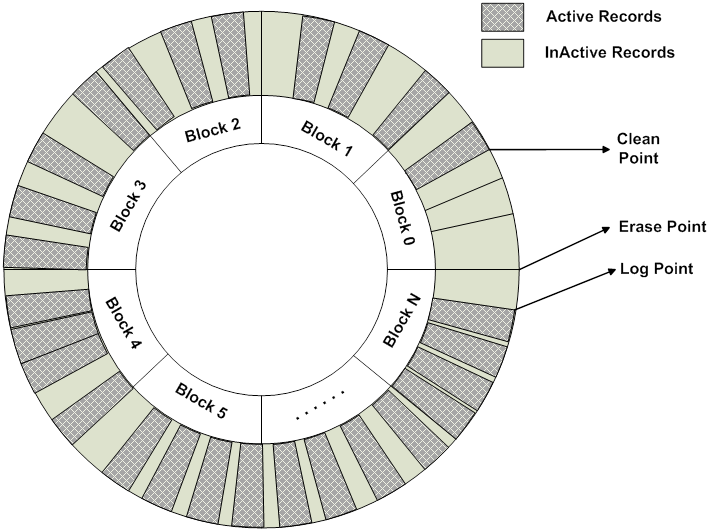
\includegraphics[width=0.48\textwidth]{C:/Ananth/OSU/CETI/MS-Thesis/MS-thesis-Report/imgs/Flash-Block-structure.png}
	\captionof{figure}{Fragmentation of blocks during steady state of the Flash device. Also shown are the Log, Clean and Erase points.}
\end{SCfigure}

The Log File System that we implement makes use of three pointers which facilitate the write operations. Log pointer always points at a location where the write operation can take place. Clean Pointer indicates the location in the Flash until which there are no active records and the Erase pointer which always moves one block at a time points at the block which was last erased. 

%-----------------------------------------------------------------------------------
\subsection{Methodology}
The GC and the applications will be implemented in Matlab 2011b. The tests were run on the Ohio Super Computer center’s cluster called Oakley. The fullness level will range from 2% to 98% and the simulations will run for 100,000 read/write accesses per fullness level. The simulations are done for all three traffic patterns for all 6 GC algorithms.

%-----------------------------------------------------------------------------------
\subsection{Implementation details:}
The application generates random records and sizes using the rand() function in Matlab. For Pareto distribution, each record is assigned a weight which decides the usage of a record. After the records are generated, based on a coin toss, it is decided whether the next operation will be a read or a write. Every time the GC is accessed, details such as amount of bytes moved, blocks erased, are captured. These details are then used to plot the required graphs. 

%-----------------------------------------------------------------------------------
\section{Related Work}



\section{Modelling}
	Efficiency of a GC is defined as the ratio of useful write vs. actual write. Useful write is defined as the amount of data passed to the write API of the file system and Actual write is the sum of amount of data moved, blocks erased and the useful write. A good GC is one which is able to find space to write data quickly. It has to do so by spreading the writes evenly across the various blocks in the flash (wear-leveling). Writing too often to a particular block can cause the flash to wear-out quickly. 

	Another important criterion in choosing a certain GC is the traffic pattern of the data. Data can be written to the flash in short bursts or can be spread out evenly. They tend to follow statistical patterns such as Uniform, Normal or Bi-Modal. For the current project, there are no sets of real-world applications which can be used to test the GC algorithms. So, one of the goals of the project is to create a set of pseudo applications which generates data that follows a Uniform, Normal or a Bi-Modal type of distribution.

Five different GC algorithms are considered which has been described below. The first two are round-robin style of GCs while the other three are generational type of algorithms.
\begin{itemize}
\item FIFE – First Insert First Erase:
The data is always written starting from the first block and when the flash reaches a pre-defined fullness level, the GC is invoked. The GC compacts the oldest block and keeps moving forward along the blocks until sufficient space is created to store the record. The GC returns an error when even after traversing the blocks, it is not able to find sufficient space. 
\item LAC – Least Active Clean:
When the GC is invoked, it finds out the block that has the least amount of active records and compacts that block. The compacted block is then used for the next write operation.
\item 3-Generation:
In this GC, the entire flash is divided into three generations. The ratio of the blocks in each generation can be 12:3:1 or 4:3:1. Data is always written to the first generation and when it becomes full, the active records are moved to the 2nd generation. When the 2nd generation becomes full, its active records are moved to the 3rd generation. This allows the GC to separate the hot from the cold data. The intuition is that this reduces the amount of movement of the active records which is a draw-back of the round-robin algorithms.
\item N-Generation:
All the blocks in the flash is considered as a generation in this algorithm. Cold data is always pushed to the highest possible generation.
\item Eta-N-Generation:
This is similar to the N-Gen algorithm, except that the amount of data that is moved is decided by a factor called Eta. Eta denotes the fullness level of the flash when the GC is invoked.
\item Gamma-N-Generation:
\end{itemize}	


The GC that will be implemented will be the one that has the best efficiency for all three traffic patterns. Depending on the outcome of this project, a single GC might be implemented or a hybrid approach will be chosen where one type of GC is used for certain fullness levels and another type for other levels of fullness.

\begin{figure}
\centering
\subfloat[]{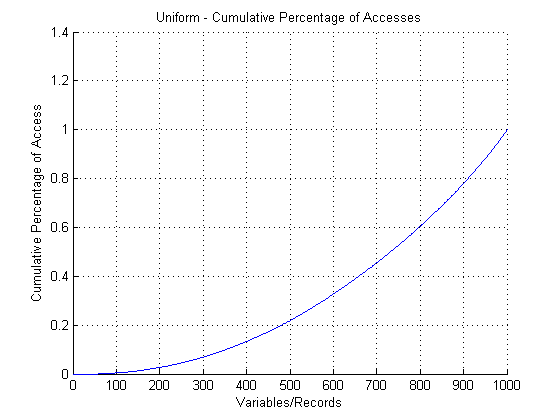
\includegraphics[width=3.1in]{C:/Ananth/OSU/CETI/MS-Thesis/MS-thesis-Report/imgs/Uniform-CumulAccess.png}} 
\subfloat[]{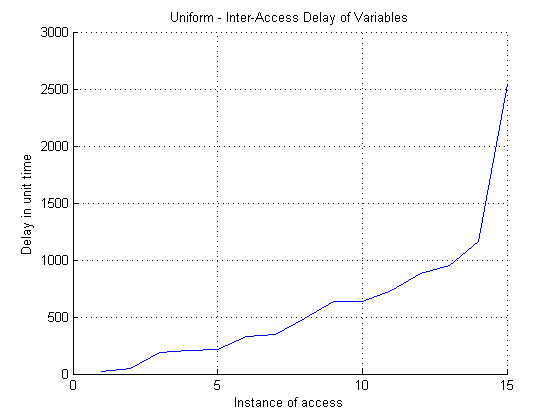
\includegraphics[width=3.1in]{C:/Ananth/OSU/CETI/MS-Thesis/MS-thesis-Report/imgs/Uniform-InterAccessDelay.png}}
\caption{Potential for 0.5 V bias.} 
\label{fig:EcUND} 
\end{figure} 

\comment{
\begin{figure}[ht]
\begin{minipage}[b]{0.4\linewidth}
\centering
	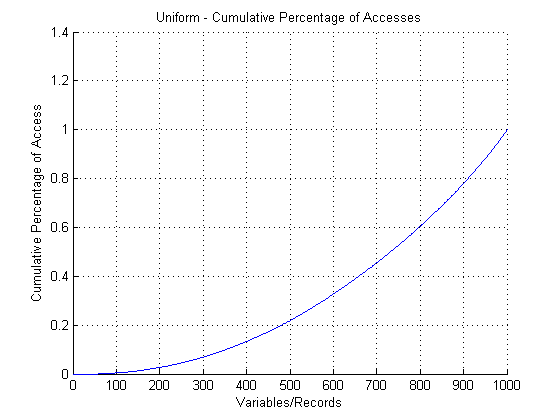
\includegraphics [width=\textwidth] {C:/Ananth/OSU/CETI/MS-Thesis/MS-thesis-Report/imgs/Uniform-CumulAccess.png}
	\captionof{figure}{Cumulative accesses for all variables that follow Uniform distribution}
	\label{UniformCumul}
\end{minipage}
\hspace{0.5cm}

\begin{minipage}[b]{0.4\linewidth}
\centering
	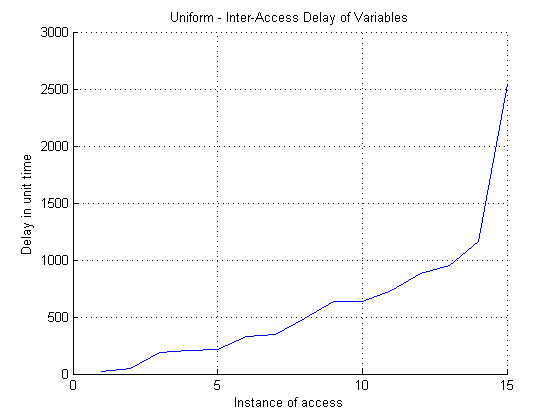
\includegraphics [width=\textwidth] {C:/Ananth/OSU/CETI/MS-Thesis/MS-thesis-Report/imgs/Uniform-InterAccessDelay.png}
	\captionof{figure}{Inter-access delay for all variables that follow Uniform distribution}
	\label{UniformCumul}
\end{minipage}
\end{figure}
}

\noindent
\begin{minipage}{\linewidth}
\makebox[\linewidth]{
    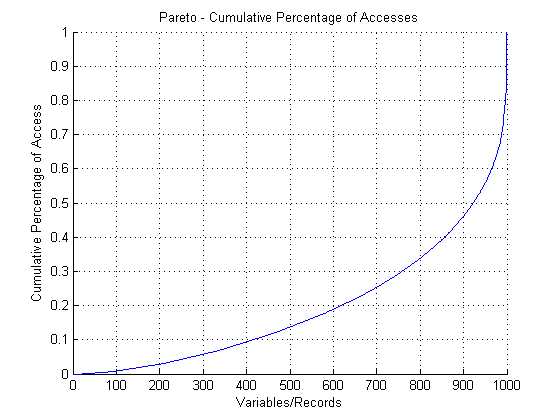
\includegraphics [keepaspectratio=true, scale = 0.6] {C:/Ananth/OSU/CETI/MS-Thesis/MS-thesis-Report/imgs/Pareto-CumulAccess.png}}
\captionof{figure}{Cumulative accesses for all variables that follow Pareto distribution}
\label{UniformCumul}
\end{minipage}

\noindent
\begin{minipage}{\linewidth}
\makebox[\linewidth]{
    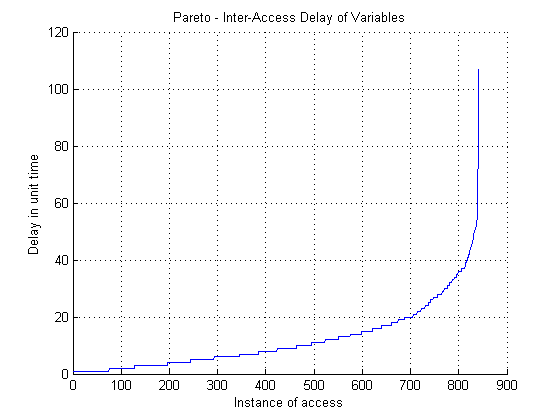
\includegraphics [keepaspectratio=true, scale = 0.6] {C:/Ananth/OSU/CETI/MS-Thesis/MS-thesis-Report/imgs/Pareto-InterAccessDelay.png}}
\captionof{figure}{Inter-access delay for all variables that follow Pareto distribution}
\label{UniformCumul}
\end{minipage}


\section{Theoretical model - FIFE Uniform}

Assumptions:\\

\begin{center}
%\captionof{table}{List of variables} 
\label{VariableList}
   \begin{tabular} {|  c | c | c | }
       \hline
	{\bf Symbol} & {\bf Explanation} & {\bf Assumption} \\ \hline
	B & Total blocks in a flash device & 128 \\ \hline
	BlockSize & The size of a block & 8192 \\ \hline
	Count of records per fullness level & N & - \\ \hline
	Average records per block & $R_b$ & - \\ \hline
	Dummy records per block & dummyRec & 1 \\ \hline
   \end{tabular}
\end{center}

Table~\ref{VariableList} shows the list of variables used. \\

%Total blocks in a flash device, B = 128\\
%The size of a block, BlockSize = 8192\\
%and let N be the count of records per fullness level.\\
%Let the count of dummy records per block be 1. dummyRec = 1 \\

The device size is, deviceSize = B * BlockSize\\
The fullness level ranges between 1\% and 98\% \\
Average number of records per block, 
\begin{equation}R_b = \frac{BlockSize}{AvgRecSize} - dummyRec\end{equation}\\


Total number of accesses is, (Number of blocks * Records per block) - (Number of records)\\
\begin{equation}NumOfAccess = ((B-1) * Rb) -  (N-1)\end{equation}\\
NumOfAccess denotes the number of accesses after which a record in a certain block is accessed again. The equation can also be written as: $((B-1) * Rb) - (B-1) * E(ARB_c)$\\
where $(B-1) * E(ARB_c)$ is the total active records in the flash, which is N.\\
\\

((B-1) * Rb) gives the total records (both active and inactive) in the entire flash and subtracting N removes the active records and leaves only the inactive. Therefore after going through the entire set of active and inactive records, we access a certain active record (hence the reason behind subtracting (N-1)). The above equation gives the best case scenario where N records are spread evenly across (B-1) blocks.\\
\\

The expectation for a record to be hit is $\frac{1}{N}$, which is the pdf for Uniform distribution. Let the probability of missing a record be denoted by $P_m$. 
\begin{equation}Pm = \frac{(N-1)}{N}\end{equation}\\
Let the expectation of active records per block that is going to be cleaned be denoted by $E(ARB_c)$\\
\\

Expectation is then, $E(ARB_c) = (P_m)^{NumOfAccess} * Rb$\\
\\
The intuition behind the equation is that, a record is missed for NumOfAccess times before it is hit. Multiplying by Rb gives the relation for all records in a certain block.\\


The expectation of the average number of records per block can be of the exponential form $1-e^{\lambda . x}$ where x is the fullness of flash (\%). To find $\lambda$ we can equate the exponential function to $R_b$ when the flash is 100\% full. 
The corresponding equation is:
$$1-e^{\lambda . x} = R_b$$
$$\lambda = \frac{log(1 - R_b)}{100}$$\\
where 100 represents the fullness of the flash in percentage.\\
\\
Expectation can therefore be given as: $$E(ARB_c) = (1 - e^{\lambda . x})$$\\
where x is the fullness of flash (\%)
\\

For a Uniform Distribution, let the total accesses to the Flash be: 100,000. Out of this, let 1/2 be writes. Hence totalWrites = 50000\\
\\

The total number of times  Garbage Collector(GC) is called decides the total move cost. During one cycle, when active records are moved from one block (x) to another (y), next invocation of the GC is related to the amount of free space in block y. Hence the relation for number of times GC is invoked is:\\
\begin{equation}NumberGCRuns = \frac{totalWrites}{(R_b - E(ARB_c))}\end{equation}\\
where ${(R_b - E(ARB_c))}$ gives the number of free slots where records can be stored.\\
\\

The fullness of the Flash is given by:
\begin{equation}FlashFullness = \frac{((N * AvgRecSize)}{deviceSize}\end{equation}\\

The expected move cost is:
\begin{equation}E(MoveCost) = E(ARB_c) * AvgRecSize * NumberGCRuns\end{equation}\\

The useful write cost is cost involved in writing data to the Flash without any overhead of moving or erasing records: \begin{equation}UsefulWriteCost = totalWrites * AvgRecSize\end{equation}\\

The actual write cost is the cost of erasing and moving records in order to write a new record:
\begin{equation}ActualWriteCost = UsefulWriteCost + ExpMoveCost\end{equation}\\

Efficiency of a Flash device is then:
\begin{equation}Efficiency = \frac{UsefulWriteCost}{ActWriteCost}\end{equation}\\

%-----------------------------------------------------------------------------------

\section{Theoretical model - FIFE Pareto}
%Assumptions:\\
%Total blocks in a flash device, B = 128\\
%The size of a block, BlockSize = 8192\\
%The device size is, deviceSize = B * BlockSize\\
%The fullness level ranges between 1\% and 98\% and let N be the count of records per fullness level.\\
%Let the count of dummy records per block be 1. dummyRec = 1\\
%Average number of records per block, 
%\begin{equation}R_b = \frac{BlockSize}{AvgRecSize} - dummyRec\end{equation}\\


Total number of accesses is, (Number of blocks * Records per block) - (Number of records)\\
\begin{equation}NumOfAccess = ((B-1) * Rb) -  (N-1)\end{equation}\\

Minimum possible value of a variable X below which it will be accessed with increased frequency
$$X_m = 0.2$$

Positive parameter for Pareto distribution is: 
$$\alpha = 1.3 $$


Average number of records per block can also be represented as, 
$$1-e^{\lambda . x} = R_b$$
$$\lambda = \frac{log(1 - R_b)}{100}$$\\
where 100 represents the fullness of the flash (\%)\\

The calculated value of $\lambda$ is used for different substitutions of x (flash fullness)  to get the expectation of active records per block that is going to be cleaned.
$$E(ARB_c) = 1-e^{\lambda . x}$$

The expectation for a record to be hit is the mean of a random variable for Pareto distribution, which is given by:\\
$$E(X) = \left\{\frac{\alpha . X_m}{\alpha - 1} \right.  if \alpha > 1$$

Therefore, expectation of a miss for Pareto distribution is:
$$P_m = 1 - \frac{\alpha . X_m}{\alpha - 1} $$

The expectation of active records in the block set to be cleaned can be assumed to be exponentially distributed. Expectation can be given as: $$E(ARB_c) = (1 - e^{\lambda . x})$$\\
where x is the fullness of flash.
\\

%-----------------------------------------------------------------------------------

\section{Theoretical model - 2-Gen Uniform}
Assumptions:\\
Average size of a record = s\\
Size of Gen1 = $F_1$\\
Size of Gen2 = $F_2$\\
\\
Total records that can be accomodated in Gen 1, $R_{gen1} = \frac{F_1}{s} $\\
\\
Total records that can be accomodated in Gen 2, $R_{gen2} = \frac{F_2}{s}$\\
\\
$X_1$ = Expectation of Active Records in Gen 1\\
$X_2$ = Expectation of Active Records in Gen 2\\
\\
Probability of a miss, $P_m = \frac{(N - 1)}{N}$\\
\\
Records moved over to Gen 2 during GC is $\delta_2$\\
Records left over in Gen 1 after GC is $\delta_1 = X_1 - \delta_2$\\
\begin{equation}X_1 = \delta_1 + \delta_2\end{equation}

\begin{equation}X_1 = {P_m}^{A_1} * R_{gen1}\end{equation}

\begin{equation}X_2 = {P_m}^{A_2} * R_{gen2}\end{equation}
\\
Count of accesses between cleans of Gen 1, $A_1 = \frac{F_1}{s} - \delta_1$\\
Count of accesses between cleans of Gen 2, $A_2 = \frac{F_2}{s} - \delta_2$\\
\\
Count of accesses between cleans of Gen 2 is, $A_2 = A_1 * R_{21}$, where $R_{21}$ is factor defined below\\
Ratio of cleans between Gen 1 and 2 is, $R_{21} = \frac{Free Space Remaining in Gen 2}{X_1}$\\
\\
Free Space remaining in Gen 2, $FS_2 = R_{gen2} - X_2$\\
Therefore, $R_{21} = \frac{FS_2}{X_1}$\\

%-----------------------------------------------------------------------------------

\section{Performance criteria}
	There are several measurements that indicate the performance of the GC algorithms. They are plotted and the different graphs that are generated are as follows:
\begin{itemize}
\item {\bf Efficiency Vs Fullness (normal scale)}
\subitem Efficiency is the primary parameter for deciding which GC is better than the rest. It denotes the amount of work done in order to write data. Lesser the work done better is the GC.
\item {\bf Efficiency Vs Fullness (log scale)}
\subitem This is the log (base 10) representation of the above graph. These denote how fast or slow efficiency of a GC changes. 
\item {\bf GC time}
\subitem Total time taken by a GC beginning from its invocation till it finds sufficient space to store a record. This is also an important criterion in deciding on a GC.
\item {\bf Fullness Vs Actual Write cost}
\subitem Actual write cost is used to calculate the Efficiency of the GC algorithm. Comparing the write cost with the erase cost and the overall efficiency helps in understanding why a given GC performs the way it does.
\end{itemize}

%#####################################################################
\section{Results}

%=====================================================================
\subsection{Uniform Distribution}
	Figure~\ref{FIFE-Uniform-EffVsFull} shows a gradual drop in efficiency for the FIFE as fullness increases. This is because as fullness increases the amount of inactive records per block decreases and the GC has to work harder to find space for new records. The corresponding figure~\ref{LAC-Uniform-EffVsFull} for LAC has almost the same pattern as that for FIFE. The figures that depict the read/write/erase costs show that majority of the work is erasing blocks which contributes the most towards the drop in efficiency.

\subsubsection{FIFE}

\begin{figure}[H]
        \centering
        \begin{subfigure}[b]{0.4\textwidth}
                \centering
                \fbox{\includegraphics[width=\textwidth]{C:/Ananth/FlashBasedFS/GC-StatisticalModel/Regular-CompactAndClean-GarbageCollector/ExecutionResults/RWAccessCnt-100000-10-21-2012-FIFE-Uniform/Plots-100000-10-21-2012-1852/EfficiencyVsFullness-10-21-2012-1852.png} }
                \caption{Efficiency Vs Fullness} \label{FIFE-Uniform-EffVsFull}
        \end{subfigure}
        ~~~ %add desired spacing between images, e. g. ~, \quad, \qquad etc. 
          %(or a blank line to force the subfigure onto a new line)
        \begin{subfigure}[b]{0.4\textwidth}
                \centering
                \fbox{\includegraphics[width=\textwidth]{C:/Ananth/FlashBasedFS/GC-StatisticalModel/Regular-CompactAndClean-GarbageCollector/ExecutionResults/RWAccessCnt-100000-10-21-2012-FIFE-Uniform/Plots-100000-10-21-2012-1852/RdWrEraseVsFullness-10-21-2012-1852.png} }
                \caption{Read, Write, Erase costs Vs Fullness} \label{FIFE-Uniform-RdWrEraseVsFull}
        \end{subfigure}
        \caption{FIFE - Uniform Distribution}
\end{figure}



\subsubsection{LAC}

\begin{figure}[H]
        \centering
        \begin{subfigure}[b]{0.4\textwidth}
                \centering
                \fbox{\includegraphics[width=\textwidth]{C:/Ananth/FlashBasedFS/GC-StatisticalModel/GenerationalGarbageCollector/LAC-Uniform/ExecutionResults/RWAccessCnt-100000-10-11-2012/Plots-100000-10-11-2012-1638/LACGC-Uniform-EffVsFull-10-11-2012-1639.png} }
                \caption{Efficiency Vs Fullness} \label{LAC-Uniform-EffVsFull}
        \end{subfigure}
        ~~~ %add desired spacing between images, e. g. ~, \quad, \qquad etc. 
          %(or a blank line to force the subfigure onto a new line)
        \begin{subfigure}[b]{0.4\textwidth}
                \centering
                \fbox{\includegraphics[width=\textwidth]{C:/Ananth/FlashBasedFS/GC-StatisticalModel/GenerationalGarbageCollector/LAC-Uniform/ExecutionResults/RWAccessCnt-100000-10-11-2012/Plots-100000-10-11-2012-1638/LACGC-Uniform-RdWrEraseVsFull-10-11-2012-1639.png} }
                \caption{Read, Write, Erase costs Vs Fullness} \label{LAC-Uniform-RdWrEraseVsFull}
        \end{subfigure}
        \caption{LAC - Uniform Distribution}
\end{figure}


\subsubsection{3-Generation}

Figure~\ref{3Gen-Uniform-EffVsFull} is almost a linear drop in efficiency. As can be observed, the drop in efficiency is much faster for 3 generation GCs when compared with FIFE algorithms. This is because the amount of blocks in the first generation is less than that in FIFE. Also, when the GC is invoked, it moves all active records from the lower to the higher generations and it has to erase the entire first generation. Even though no effort is spent in moving around active records at regular intervals, the overall effort vs writing a new record is much more than that in FIFE.

\begin{figure}[H]
        \centering
        \begin{subfigure}[b]{0.4\textwidth}
                \centering
                \fbox{\includegraphics[width=\textwidth]{C:/Ananth/FlashBasedFS/GC-StatisticalModel/GenerationalGarbageCollector/3Gen-Uniform-FINAL/ExecutionResults/RWAccessCnt-100000-9-8-2012-3Gen-Uniform-64-48-16/Plots-100000-9-8-2012-735/3GEN-Uniform-EffVsFull-9-8-2012-735.png} }
                \caption{Efficiency Vs Fullness} \label{3Gen-Uniform-EffVsFull}
        \end{subfigure}
        ~~~ %add desired spacing between images, e. g. ~, \quad, \qquad etc. 
          %(or a blank line to force the subfigure onto a new line)
        \begin{subfigure}[b]{0.4\textwidth}
                \centering
                \fbox{\includegraphics[width=\textwidth]{C:/Ananth/FlashBasedFS/GC-StatisticalModel/GenerationalGarbageCollector/3Gen-Uniform-FINAL/ExecutionResults/RWAccessCnt-100000-9-8-2012-3Gen-Uniform-64-48-16/Plots-100000-9-8-2012-735/3GEN-Uniform-RdWrEraseVsFull-9-8-2012-735.png} }
                \caption{Read, Write, Erase costs Vs Fullness} \label{3Gen-Uniform-RdWrEraseVsFull}
        \end{subfigure}
        \caption{3Gen - Uniform Distribution}
\end{figure}


\subsubsection{N-Generation}

Figure~\ref{NGen-Uniform-EffVsFull} shows a sharp drop in efficiency even at lower fullness levels. This is because only one block is used for writing new records and the GC has to move records to higher generations to make space for new incoming records. Ideally this algorithm should have high efficiency for data with high locality of reference. We conducted a few experiments on this premise by generating data that has high locality of reference. But even in that case, we observed a similar behaviour. This is again due to the fact that there is very little space for writing new records.

\begin{figure}[H]
        \centering
        \begin{subfigure}[b]{0.4\textwidth}
                \centering
                \fbox{\includegraphics[width=\textwidth]{C:/Ananth/FlashBasedFS/GC-StatisticalModel/GenerationalGarbageCollector/NGen-Uniform-FINAL/ExecutionResults/ExecutionResults/RWAccessCnt-100000-8-15-2012/Plots-100000-8-15-2012-1526/NGEN-Uniform-EffVsFull-8-15-2012-1526.png} }
                \caption{Efficiency Vs Fullness} \label{NGen-Uniform-EffVsFull}
        \end{subfigure}
        ~~~ %add desired spacing between images, e. g. ~, \quad, \qquad etc. 
          %(or a blank line to force the subfigure onto a new line)
        \begin{subfigure}[b]{0.4\textwidth}
                \centering
                \fbox{\includegraphics[width=\textwidth]{C:/Ananth/FlashBasedFS/GC-StatisticalModel/GenerationalGarbageCollector/NGen-Uniform-FINAL/ExecutionResults/ExecutionResults/RWAccessCnt-100000-8-15-2012/Plots-100000-8-15-2012-1526/NGEN-Uniform-RdWrEraseVsFull-8-15-2012-1526.png} }
                \caption{Read, Write, Erase costs Vs Fullness} \label{NGen-Uniform-RdWrEraseVsFull}
        \end{subfigure}
        \caption{NGen - Uniform Distribution}
\end{figure}


%---------------------------------------------------------------------------------------------------------------------------------------
\subsection{Pareto Distribution}

\subsubsection{FIFE}

Figures~\ref{FIFE-Pareto-EffVsFull}~\ref{LAC-Pareto-EffVsFull} are similar to those for Uniform Distribution, except that at lower fullness levels, the drop in efficiency is much faster. This is due to the cost involved in moving records that are ``cold''. In Uniform, there is a higher chance for every record to be invalidated, whereas in Pareto, few records are inactivated more often. Pareto distribution has more ``cold'' data than Uniform and hence contributes more towards the move cost. 

\begin{figure}[H]
        \centering
        \begin{subfigure}[b]{0.4\textwidth}
                \centering
                \fbox{\includegraphics[width=\textwidth]{C:/Ananth/FlashBasedFS/GC-StatisticalModel/Regular-CompactAndClean-GarbageCollector/ExecutionResults/RWAccessCnt-100000-10-21-2012-FIFE-Pareto/Plots-100000-10-21-2012-191/EfficiencyVsFullness-10-21-2012-191.png} }
                \caption{Efficiency Vs Fullness} \label{FIFE-Pareto-EffVsFull}
        \end{subfigure}
        ~~~ %add desired spacing between images
        \begin{subfigure}[b]{0.4\textwidth}
                \centering
                \fbox{\includegraphics[width=\textwidth]{C:/Ananth/FlashBasedFS/GC-StatisticalModel/Regular-CompactAndClean-GarbageCollector/ExecutionResults/RWAccessCnt-100000-10-21-2012-FIFE-Pareto/Plots-100000-10-21-2012-191/RdWrEraseVsFullness-10-21-2012-191.png} }
                \caption{Read, Write, Erase costs Vs Fullness} \label{FIFE-Pareto-RdWrEraseVsFull}
        \end{subfigure}
        \caption{FIFE - Pareto Distribution}
\end{figure}


\subsubsection{LAC}

\begin{figure}[H]
        \centering
        \begin{subfigure}[b]{0.4\textwidth}
                \centering
                \fbox{\includegraphics[width=\textwidth]{C:/Ananth/FlashBasedFS/GC-StatisticalModel/GenerationalGarbageCollector/LAC-Pareto/ExecutionResults/RWAccessCnt-100000-10-11-2012-LAC-Pareto/Plots-100000-10-11-2012-1621/LACGC-Pareto-EffVsFull-10-11-2012-1621.png} }
                \caption{Efficiency Vs Fullness} \label{LAC-Pareto-EffVsFull}
        \end{subfigure}
        ~~~ %add desired spacing between images
        \begin{subfigure}[b]{0.4\textwidth}
                \centering
                \fbox{\includegraphics[width=\textwidth]{C:/Ananth/FlashBasedFS/GC-StatisticalModel/GenerationalGarbageCollector/LAC-Pareto/ExecutionResults/RWAccessCnt-100000-10-11-2012-LAC-Pareto/Plots-100000-10-11-2012-1621/LACGC-Pareto-RdWrEraseVsFull-10-11-2012-1621.png} }
                \caption{Read, Write, Erase costs Vs Fullness} \label{LAC-Pareto-RdWrEraseVsFull}
        \end{subfigure}
        \caption{LAC - Pareto Distribution}
\end{figure}


\subsubsection{Generational}

Figures~\ref{3Gen-Pareto-EffVsFull}~\ref{NGen-Pareto-EffVsFull}~\ref{Eta-NGen-Pareto-EffVsFull} show a similar behaviour to that of Uniform distribution. These set of graphs are counter-intuitive and therefore have to be analyzed a little deeper. For instance, in 3-Generation GC, when the first generation becomes full and when the GC is invoked, the active records in Gen-1 are moved to Gen-2. This pattern continues and at steady state, Gen-2 has both active and inactive records and Gen-3 also has the same, but has a higher distribution of active records. Though more space is created during one cycle of GC, the cost per GC over the life-time of the flash is almost the same for Pareto and for Uniform. Therefore, we decided not to consider erase cost, but only the move cost. 

\begin{figure}[H]
        \centering
        \begin{subfigure}[b]{0.4\textwidth}
                \centering
                \fbox{\includegraphics[width=\textwidth]{C:/Ananth/FlashBasedFS/GC-StatisticalModel/GenerationalGarbageCollector/3Gen-Pareto-FINAL/ExecutionResults/RWAccessCnt-200000-9-8-2012-3Gen-Pareto-64-48-16-200K/Plots-200000-9-8-2012-35/3Gen-Pareto-EffVsFull-9-8-2012-36.png} }
                \caption{Efficiency Vs Fullness} \label{3Gen-Pareto-EffVsFull}
        \end{subfigure}
        ~~~ %add desired spacing between images
        \begin{subfigure}[b]{0.4\textwidth}
                \centering
                \fbox{\includegraphics[width=\textwidth]{C:/Ananth/FlashBasedFS/GC-StatisticalModel/GenerationalGarbageCollector/3Gen-Pareto-FINAL/ExecutionResults/RWAccessCnt-200000-9-8-2012-3Gen-Pareto-64-48-16-200K/Plots-200000-9-8-2012-35/3Gen-Pareto-RdWrEraseVsFull-9-8-2012-36.png} }
                \caption{Read, Write, Erase costs Vs Fullness} \label{3Gen-Pareto-RdWrEraseVsFull}
        \end{subfigure}
        \caption{3Gen - Pareto Distribution}
\end{figure}




\begin{figure}[H]
        \centering
        \begin{subfigure}[b]{0.4\textwidth}
                \centering
                \fbox{\includegraphics[width=\textwidth]{C:/Ananth/FlashBasedFS/GC-StatisticalModel/GenerationalGarbageCollector/NGen-Pareto-FINAL/ExecutionResults/RWAccessCnt-100000-9-17-2012-NGen-Pareto/Plots-100000-9-17-2012-559/NGen-Pareto-EffVsFull-9-17-2012-60.png} }
                \caption{Efficiency Vs Fullness} \label{NGen-Pareto-EffVsFull}
        \end{subfigure}
        ~~~ %add desired spacing between images
        \begin{subfigure}[b]{0.4\textwidth}
                \centering
                \fbox{\includegraphics[width=\textwidth]{C:/Ananth/FlashBasedFS/GC-StatisticalModel/GenerationalGarbageCollector/NGen-Pareto-FINAL/ExecutionResults/RWAccessCnt-100000-9-17-2012-NGen-Pareto/Plots-100000-9-17-2012-559/NGen-Pareto-RdWrEraseVsFull-9-17-2012-60.png} }
                \caption{Read, Write, Erase costs Vs Fullness} \label{NGen-Pareto-RdWrEraseVsFull}
        \end{subfigure}
        \caption{NGen - Pareto Distribution}
\end{figure}



\begin{figure}[H]
        \centering
        \begin{subfigure}[b]{0.4\textwidth}
                \centering
                \fbox{\includegraphics[width=\textwidth]{C:/Ananth/FlashBasedFS/GC-StatisticalModel/GenerationalGarbageCollector/ETANGen-Pareto-FINAL/ExecutionResults/RWAccessCnt-100000-9-16-2012-ETA-Pareto/Plots-100000-9-16-2012-2153/ETA-NGen-Pareto-Actual-EffVsFull-9-16-2012-2153.png} }
                \caption{Efficiency Vs Fullness} \label{Eta-NGen-Pareto-EffVsFull}
        \end{subfigure}
        ~~~ %add desired spacing between images
        \begin{subfigure}[b]{0.4\textwidth}
                \centering
                \fbox{\includegraphics[width=\textwidth]{C:/Ananth/FlashBasedFS/GC-StatisticalModel/GenerationalGarbageCollector/ETANGen-Pareto-FINAL/ExecutionResults/RWAccessCnt-100000-9-16-2012-ETA-Pareto/Plots-100000-9-16-2012-2153/ETA-NGen-Pareto-Actual-RdWrEraseVsFull-9-16-2012-2153.png} }
                \caption{Read, Write, Erase costs Vs Fullness} \label{Eta-NGen-Pareto-RdWrEraseVsFull}
        \end{subfigure}
        \caption{Eta-NGen - Pareto Distribution}
\end{figure}


%---------------------------------------------------------------------------------------------------------------------------------------
%\subsection{BiModal Distribution}
%	No individual graphs generated.


%====================================================================
\subsection{Efficiency Vs Fullness - Combined Graphs}

Figures~\ref{Uniform-AllGC-EffVsFull}~\ref{Pareto-AllGC-EffVsFull}~\ref{BiModal-AllGC-EffVsFull} show the plots for the various GCs. As can be observed, the Round-Robin style of algorithms occupy the top half of the chart and the generational algorithms occupying the bottom half. The 3-Gen algorithm comes in the middle of the chart. The reason behind this has been mentioned in the previous results.

\subsubsection{Uniform Distribution}

\begin{figure}[H]
        \centering
        \begin{subfigure}[b]{0.4\textwidth}
                \centering
                \fbox{\includegraphics[width=\textwidth]{C:/Ananth/FlashBasedFS/GC-StatisticalModel/DesignDocument/FinalPresentation/Uniform/Plots-Uniform-1013/EffVsFull-220.png} }
                \caption{Efficiency Vs Fullness} \label{Uniform-AllGC-EffVsFull}
        \end{subfigure}
        ~~~ %add desired spacing between images
        \begin{subfigure}[b]{0.4\textwidth}
                \centering
                \fbox{\includegraphics[width=\textwidth]{C:/Ananth/FlashBasedFS/GC-StatisticalModel/DesignDocument/FinalPresentation/Uniform/Plots-Uniform-1013/GC-Time-220.png} }
                \caption{Time Taken by GCs Vs Fullness} \label{Uniform-GCTimeVsFull}
        \end{subfigure}
        \caption{Uniform Distribution-Efficiency Vs Fullness for all GCs}
\end{figure}

\subsubsection{Pareto Distribution}

\begin{figure}[H]
        \centering
        \begin{subfigure}[b]{0.4\textwidth}
                \centering
                \fbox{\includegraphics[width=\textwidth]{C:/Ananth/FlashBasedFS/GC-StatisticalModel/DesignDocument/FinalPresentation/Pareto/Plots-Pareto-1013/EffVsFull-114.png} }
                \caption{Efficiency Vs Fullness} \label{Pareto-AllGC-EffVsFull}
        \end{subfigure}
        ~~~ %add desired spacing between images
        \begin{subfigure}[b]{0.4\textwidth}
                \centering
                \fbox{\includegraphics[width=\textwidth]{C:/Ananth/FlashBasedFS/GC-StatisticalModel/DesignDocument/FinalPresentation/Pareto/Plots-Pareto-1013/GC-Time-116.png} }
                \caption{Time Taken by GCs Vs Fullness} \label{Pareto-GCTimeVsFull}
        \end{subfigure}
        \caption{Pareto Distribution-Efficiency Vs Fullness for all GCs}
\end{figure}

\subsubsection{BiModal Distribution}

\begin{figure}[H]
        \centering
        \begin{subfigure}[b]{0.4\textwidth}
                \centering
                \fbox{\includegraphics[width=\textwidth]{C:/Ananth/FlashBasedFS/GC-StatisticalModel/DesignDocument/FinalPresentation/BiModal/Plots-BiModal-1013/EffVsFull-224.png} }
                \caption{Efficiency Vs Fullness} \label{BiModal-AllGC-EffVsFull}
        \end{subfigure}
        ~~~ %add desired spacing between images
        \begin{subfigure}[b]{0.4\textwidth}
                \centering
                \fbox{\includegraphics[width=\textwidth]{C:/Ananth/FlashBasedFS/GC-StatisticalModel/DesignDocument/FinalPresentation/BiModal/Plots-BiModal-1013/GC-Time-225.png} }
                \caption{Time Taken by GCs Vs Fullness} \label{BiModal-GCTimeVsFull}
        \end{subfigure}
        \caption{BiModal Distribution-Efficiency Vs Fullness for all GCs}
\end{figure}


%====================================================================
\subsection{Theoretical and Simulation results - Uniform Distribution - with different percentages of access}
	Combination of theoretical and simulation results. Attempts to beat FIFE's efficiency by generational algorithms by accessing 20\%, 40\%, 60\%, 80\% and 100\% of the records.	

\begin{figure}[H]
        \centering
        \begin{subfigure}[b]{0.4\textwidth}
                \centering
                \fbox{\includegraphics[width=2.8in, height=1.8in]{C:/Ananth/FlashBasedFS/GC-StatisticalModel/Regular-CompactAndClean-GarbageCollector/Theoritical-Plots/Plots-Dec16/FIFE-simulation-theoretical-Dec16/EfficiencyVsFullness.png} }
                \caption{Shows the Efficiency vs Fullness plot for FIFE GC algorithm. It includes the theoretical plot as well} \label{FIFE-AllGC-AllAccess-EffVsFull}
        \end{subfigure}
        ~~~ %add desired spacing between images
        \begin{subfigure}[b]{0.4\textwidth}
                \centering
                \fbox{\includegraphics[width=2.8in, height=1.8in]{C:/Ananth/FlashBasedFS/GC-StatisticalModel/Regular-CompactAndClean-GarbageCollector/Theoritical-Plots/Plots-Dec16/1Gen-simulation-theoretical-Dec16/EfficiencyVsFullness.png} }
                \caption{Shows the Efficiency vs Fullness plot for 1Gen GC algorithm. It includes the theoretical plot as well} \label{1Gen-AllGC-AllAccess-EffVsFull}
        \end{subfigure}
        ~~~ %add desired spacing between images
        \centering
        \begin{subfigure}[b]{0.4\textwidth}
                \centering
                \fbox{\includegraphics[width=2.8in, height=1.8in]{C:/Ananth/FlashBasedFS/GC-StatisticalModel/Regular-CompactAndClean-GarbageCollector/Theoritical-Plots/Plots-Dec16/2Gen-simulation-theoretical-Dec16/EfficiencyVsFullness.png} }
                \caption{Shows the Efficiency vs Fullness plot for 2Gen GC algorithm. It includes the theoretical plot as well} \label{2Gen-AllGC-AllAccess-EffVsFull}
        \end{subfigure}
        ~~~ %add desired spacing between images
        \begin{subfigure}[b]{0.4\textwidth}
                \centering
                \fbox{\includegraphics[width=2.8in, height=1.8in]{C:/Ananth/FlashBasedFS/GC-StatisticalModel/Regular-CompactAndClean-GarbageCollector/Theoritical-Plots/Plots-Dec16/3Gen-simulation-theoretical-Dec18/EfficiencyVsFullness.png} }
                \caption{Shows the Efficiency vs Fullness plot for 3Gen GC algorithm. It includes the theoretical plot as well} \label{3Gen-AllGC-AllAccess-EffVsFull}
        \end{subfigure}
        ~~~ %add desired spacing between images
        \centering
        \begin{subfigure}[b]{0.4\textwidth}
                \centering
                \fbox{\includegraphics[width=2.8in, height=1.8in]{C:/Ananth/FlashBasedFS/GC-StatisticalModel/Regular-CompactAndClean-GarbageCollector/Theoritical-Plots/Plots-Dec16/NGen-simulation-theoretical-Dec20/EfficiencyVsFullness.png} }
                \caption{Shows the Efficiency vs Fullness plot for NGen GC algorithm. It includes the theoretical plot as well} \label{NGen-AllGC-AllAccess-EffVsFull}
        \end{subfigure}
        \caption{Theoretical and Simulation results - Uniform Distribution - with different percentages of access}
\end{figure}

%====================================================================




\section{Simulations}

%-----------------------------------------------------------------------------------

\subsection*{Summary}




\nocite{Rosenblum91}
\nocite{Chang05}
\nocite{Parker03}

\bibliographystyle{unsrt}
\bibliography{References}


\end{document}
